% -*- latex -*-
%%%%%%%%%%%%%%%%%%%%%%%%%%%%%%%%%%%%%%%%%%%%%%%%%%%%%%%%%%%%%%%%
%%%%%%%%%%%%%%%%%%%%%%%%%%%%%%%%%%%%%%%%%%%%%%%%%%%%%%%%%%%%%%%%
%%%%
%%%% This text file is part of the source of 
%%%% `Parallel Computing'
%%%% by Victor Eijkhout, copyright 2012/3/4/5
%%%%
%%%%%%%%%%%%%%%%%%%%%%%%%%%%%%%%%%%%%%%%%%%%%%%%%%%%%%%%%%%%%%%%
%%%%%%%%%%%%%%%%%%%%%%%%%%%%%%%%%%%%%%%%%%%%%%%%%%%%%%%%%%%%%%%%

%\input chapters/mpi-idiom-comm
\Level 0 {Subcommunications}

In many scenarios you divide a large job over all the available processors.
However, your job has two or more parts that can be considered as
jobs by themselves. In that case it makes sense to divide your processors
into subgroups accordingly.

Supose for instance that you are running a simulation where inputs are generated,
a~computation is performed on them, and the results of this computation
are analyzed or rendered graphically. You could then consider dividing your
processors in three groups corresponding to generation, computation, rendering.

As long as you only do sends and receives, this division works fine. However,
if one group of processes needs to perform a collective operation, you don't
want the other groups involved in this. Thus, you really want the three groups
to be really distinct from each other.

In order to make such subsets of processes, MPI has the mechanism of
taking a subset of \indexmpishow{MPI_COMM_WORLD} and turning that subset
into a new communicator.

Now you understand why the MPI collective calls had an argument for the
communicator: a~collective involves all proceses \emph{of that communicator}.
By making a communicator that contains a subset of all available processes,
you can do a collective on that subset.

\Level 1 {Scenario: climate model}

A climate simulation code has several components, for instance corresponding
to land, air, ocean, and ice. You can imagine that each needs a different set
of equations and algorithms to simulate. You can then divide your processes,
where each subset simulates one component of the climate, occasionally communicating
with the other components.

\Level 1 {Scenario: quicksort}

The popular quicksort algorithm works by splitting the data
into two subsets that each can be sorted individually.
If you want to sort in parallel, you could implement this by making two subcommunicators,
and sorting the data on these, creating recursively more subcommunicators.

%\input chapters/mpi-intro-comm
\Level 0 {Communicators}
\commandref{communicators}
\index{communicator|(}

A communicator is an object describing a group of processes. In many 
applications all processes work together closely coupled, and the
only communicator you need is \n{MPI_COMM_WORLD}. However, there are 
circumstances where you want one subset of processes to operate 
independently of another subset. For example:
\begin{itemize}
\item If processors are organized in a $2\times2$ grid, you may want
  to do broadcasts inside a row or column. 
\item For an application that includes a producer and a consumer part,
  it makes sense to split the processors accordingly.
\end{itemize}
In this section we will see mechanisms for defining new communicators
and sending messages between communicators.

An important reason for using communicators is the development of
software libraries. If the routines in a library use their own communicator
(even if it is a duplicate of the `outside' communicator), there
will never be a confusion between message tags inside and outside the 
library.

\Level 1 {Basics}

There are three predefined communicators:
\begin{itemize}
\item \indexmpishow{MPI_COMM_WORLD} comprises all processes that were started 
  together by \indexterm{mpirun} (or some related program).
\item \indexmpishow{MPI_COMM_SELF} is the communicator that contains only
   the current process.
\item \indexmpishow{MPI_COMM_NULL} is the invalid communicator. Routines
  that construct communicators can give this as result if an error occurs.
\end{itemize}
%Implementationally, communicators are integers, so you can use a 
%simple test for equality.

In some applications you will find yourself regularly creating new
communicators, using the mechanisms described below. In that case, you
should de-allocate communicators with \indexmpishow{MPI_Comm_free} when
you're done with them.

\Level 1 {Creating new communicators}

There are various ways of making new communicators. We discuss three 
mechanisms, from simple to complicated.

\Level 2 {Duplicating communicators}
\commandref{comm-dup}

With \indexmpishow{MPI_Comm_dup} you can make an exact duplicate of a communicator.
This may seem pointless, but it is actually very useful for the design of
software libraries. Image that you have a code
\begin{verbatim}
MPI_Isend(...); MPI_Irecv(...);
// library call
MPI_Waitall(...);
\end{verbatim}
and suppose that the library has receive calls. Now it is possible that the 
receive in the library inadvertently
catches the message that was sent in the outer environment.

To prevent this confusion, the library should duplicate the outer communicator,
and send all messages with respect to its duplicate. Now messages from the user
code can never reach the library software, since they are on different communicators.

\Level 2 {Splitting a communicator}
\commandref{comm-split}

Splitting a communicator into multiple disjoint communicators
can be done with \indexmpishow{MPI_Comm_split}.
This uses a `colour':
\begin{verbatim}
MPI_Comm_split( old_comm, colour, new_comm, .... );
\end{verbatim}
  and all processes in the old communicator with the same colour
  wind up in a new communicator together. The old communicator still exists,
  so processes now have two different contexts in which to communicate.

Here is one example of communicator splitting. Suppose your processors
are in a two-dimensional grid:
\begin{verbatim}
MPI_Comm_rank( MPI_COMM_WORLD, &mytid );
proc_i = mytid % proc_column_length;
proc_j = mytid / proc_column_length;
\end{verbatim}
You can now create a communicator per column:
\begin{verbatim}
MPI_Comm column_comm;
MPI_Comm_split( MPI_COMM_WORLD, proc_j, mytid, &column_comm );
\end{verbatim}
and do a broadcast in that column:
\begin{verbatim}
MPI_Bcast( data, /* tag: */ 0, column_comm );
\end{verbatim}
Because of the SPMD nature of the program, you are now doing in parallel
a broadcast in every processor column. Such operations often appear
in \indexterm{dense linear algebra}.

As an example of communicator splitting, consider the recursive
algorithm for \indextermbus{matrix}{transposition}.
Processors are organized in a square grid. The matrix is divided
on $2\times 2$ block form:
%
\begin{figure}
  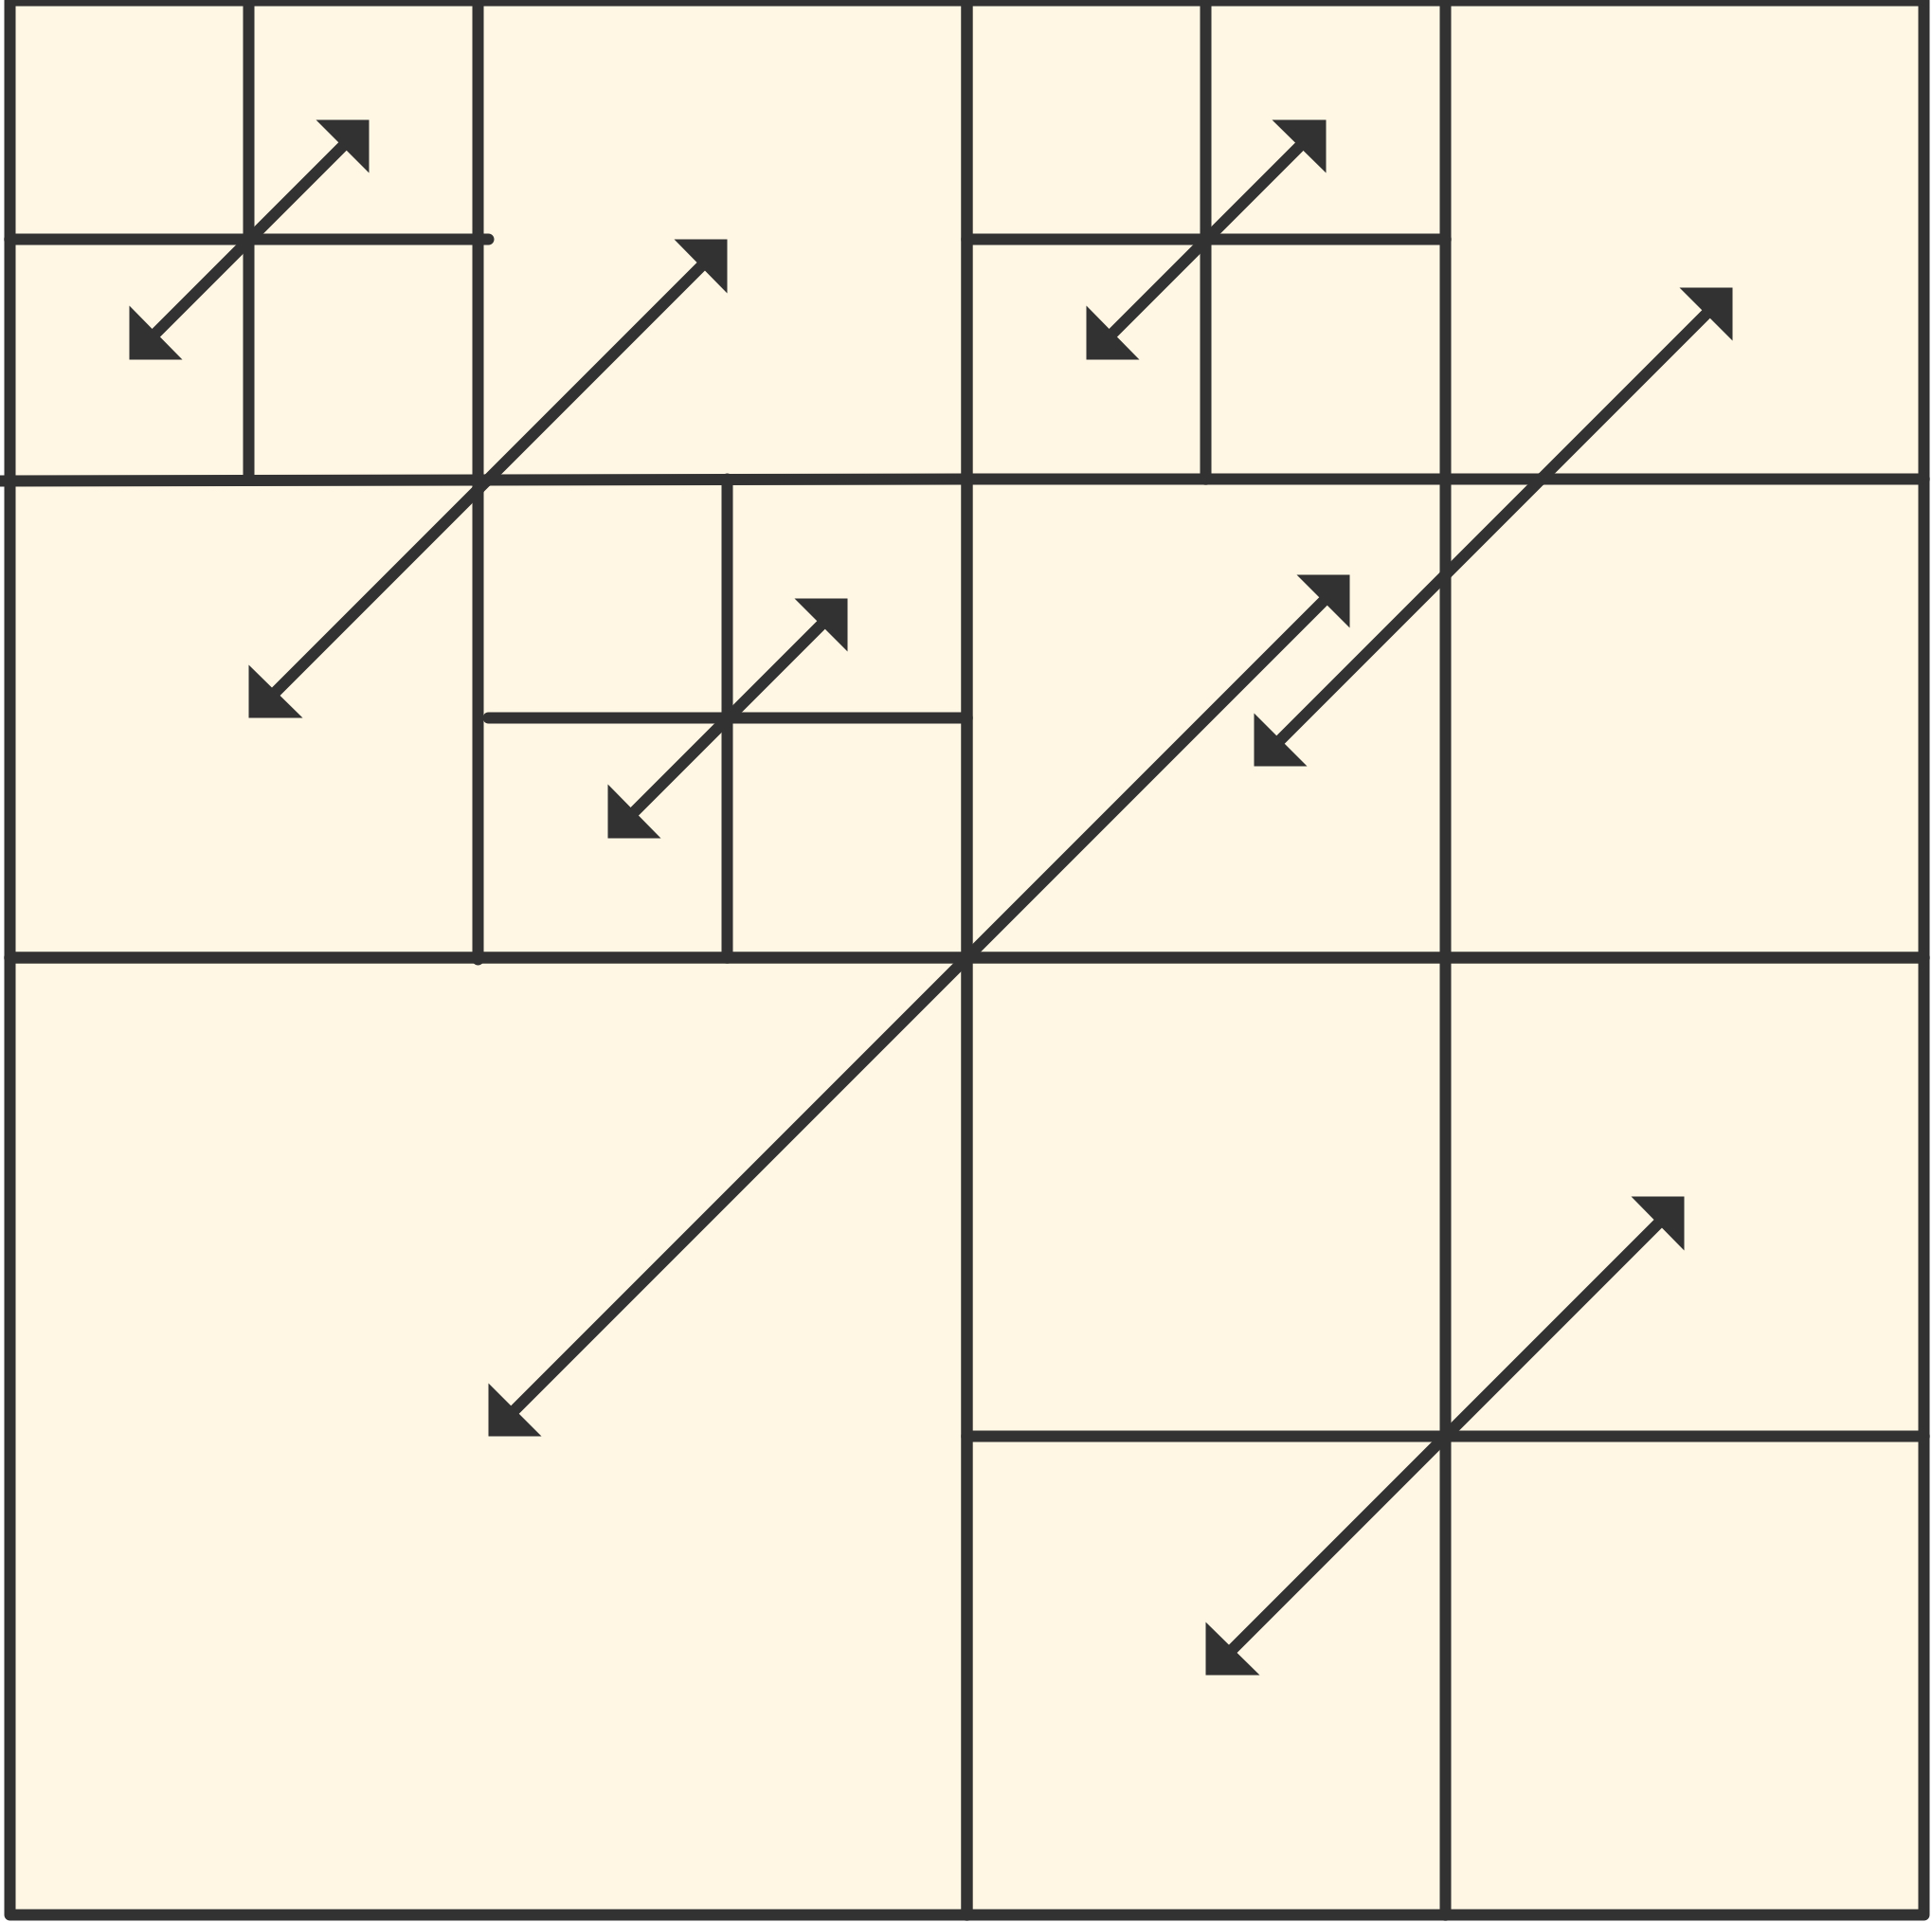
\includegraphics[scale=.1]{recursive-transpose}
  \caption{Recursive algorithm for matrix transposition}
  \label{fig:recursive-transpose}
\end{figure}
%
\begin{itemize}
\item Swap blocks $(1,2)$ and $(2,1)$; then
\item Divide the processors into four subcommunicators, and
  apply this algorithm recursively on each;
\item If the communicator has only one process, transpose the matrix in place.
\end{itemize}
See figure~\ref{fig:recursive-transpose}.

There is an important application of communicator splitting in the
context of one-sided communication, grouping processes by whether they
access the same shared memory area; see section~\ref{mpi-comm-split-type}.

\Level 2 {Process groups}

The most general mechanism is based on groups: you can extract the
group from a communicator, combine different groups, and form a new
communicator from the resulting group.

The group mechanism is more involved. You get the group from a
communicator, or conversely make a communicator from a group with
\indexmpishow{MPI_Comm_group} and \indexmpishow{MPI_Comm_create}:
\begin{verbatim}
MPI_Comm_group( comm, &group);
MPI_Comm_create( old_comm, group, &new_comm );
\end{verbatim}
and groups are manipulated with
\indexmpishow{MPI_Group_incl}, \indexmpishow{MPI_Group_excl},
\indexmpishow{MPI_Group_difference} and a few more.

You can name your communicators with \indexmpishow{MPI_Comm_set_name}, which
could improve the quality of error messages when they arise.

\Level 1 {Intra-communicators}
\label{sec:comm-group}

We start by exploring the mechanisms for creating a communicator that
encompasses a subset of \n{MPI_COMM_WORLD}. 

The most general mechanism for creating communicators is through
process groups: you can query the group of processes of a
communicator, manipulate groups, and make a new communicator out of a
group you have formed.

\begin{verbatim}
MPI_COMM_GROUP (comm, group, ierr)
MPI_COMM_CREATE (MPI_Comm comm,MPI_Group group, MPI_Comm newcomm, ierr)
\end{verbatim}

\begin{verbatim}
MPI_GROUP_UNION(group1, group2, newgroup, ierr)
MPI_GROUP_INTERSECTION(group1, group2, newgroup, ierr)
MPI_GROUP_DIFFERENCE(group1, group2, newgroup, ierr)
\end{verbatim}

\begin{verbatim}
MPI_GROUP_INCL(group, n, ranks, newgroup, ierr)
MPI_GROUP_EXCL(group, n, ranks, newgroup, ierr)
\end{verbatim}
\begin{verbatim}
MPI_GROUP_SIZE(group, size, ierr)
MPI_GROUP_RANK(group, rank, ierr)
\end{verbatim}

\Level 1 {Inter-communicators}

If two disjoint communicators exist, it may be necessary to
communicate between them. This can of course be done by creating a new
communicator that overlaps them, but this would be complicated: since
the `inter' communication happens in the overlap communicator, you
have to translate its ordering into those of the two worker
communicators. It would be easier to express messages directly in
terms of those communicators, and this can be done with
`inter-communicators'.

\begin{verbatim}
MPI_Intercomm_create (local_comm, local_leader, bridge_comm, remote_leader, tag, newintercomm, ierr)
\end{verbatim}
After this, the intercommunicator can be used in collectives such as
\begin{verbatim}
MPI_Bcast (buff, count, dtype, root, comm, ierr)
\end{verbatim}
\begin{itemize}
\item In group~A, the root process passes \n{MPI_ROOT} as
  `root' value; all others use \n{MPI_NULL_PROC}.
\item In group~B, all processes use a `root' value that is the
  rank of the root process in the root group.
\end{itemize}
Gather and scatter behave similarly; the allgather is different: all
send buffers of group~A are concatenated in rank order, and places on
all processes of group~B.

Inter-communicators can be used if two groups of process work
asynchronously with respect to each other; another application is
fault tolerance (section~\ref{mpi:tolerant}).

\Level 1 {Process topologies}
\commandref{topology}

In the communicators you have seen so far, processes are linearly ordered.
In some circumstances the problem you are coding has some structure,
and expressing the program
in terms of that structure would be convenient. For this purpose, MPI 
can define a virtual \indexterm{topology}. There are two types:
\begin{itemize}
\item regular, Cartesian, grids; and
\item general graphs.
\end{itemize}

\Level 2 {Cartesian grid topology}
\commandref{cartesian}

A \indextermsub{Cartesian}{grid} is a structure, typically in 2~or~3 dimensions,
of points that have two neighbours in each of the dimensions.
Thus, if a Cartesian grid has sizes $K\times M\times N$, its
points have coordinates $(k,m,n)$ with $0\leq k<K$ et cetera.
Most points have six neighbours $(k\pm1,m,n)$, $(k,m\pm1,n)$, $(k,m,n\pm1)$;
the exception are the edge points. A~grid where edge processors
are connected through \indexterm{wraparound connections} is called
a \indextermsub{periodic}{grid}.

The most common use of Cartesian coordinates
is to find the rank of process by referring to it in grid terms.
For instance, one could ask `what are my neighbours offset by $(1,0,0)$, 
$(-1,0,0)$, $(0,1,0)$ et cetera'.

\index{communicator|)}

